\chapter{Поиск гигантских вспышек от мягких гамма-репитеров в ближайших галактиках 
         среди коротких всплесков Конус-Винд} \label{chapt4}
Мягкие гамма-репитеры (SGR) относятся к редкому классу нейтронных звёзд, проявляющих 
два типа активности в жестком рентгеновском диапазоне ($\sim 10\textrm{--}1000$~кэВ). 
Во время периода активности SGR испускают короткие ($\sim0.001\textrm{--}1$~c) жесткие рентгеновские всплески 
с пиковой светимостью $10^{38}\textrm{--}10^{42}$~эрг~с$^{-1}$. Фаза активности может длится 
от дней до года, после чего наступает длительная фаза затишья. Значительно реже, 
возможно один раз за время нахождения нейтронной звезды в стадии SGR, SGR может 
производить гигантские вспышки (ГВ), во время которых высвобождается значительная 
энергия $\sim(0.01\textrm{--}1)\times 10^{46}$~эрг. Гигантская вспышка начинается 
с короткого $\sim 0.2\textrm{--}0.5$~с жесткого импульса с быстрым нарастанием и 
более медленным спаданием и пиковой светимостью до $\sim 10^{47}$~эрг~с$^{-1}$, который переходит 
в длинный затухающий хвост, модулированный вращением нейтронной звезды. 
Подробное описание наблюдательных свойств SGR дано в работе~\citep{Mereghetti2013}.

К настоящему моменту известно 15 SGR~\citep{Olausen_Kaspi2014}, из которых 14 
находятся в нашей Галактике и один расположен в Большом Магеллановом Облаке. 

Первая гигантская вспышка была зарегистрирована от SGR в Большом Магеллановом Облаке 
5~марта 1979~года приборами Конус на советских межпланетных станциях 
Венера~\citep{Golenetskii1979SvAL, Mazets1979} 
и сетью IPN~\citep{Barat1979, Cline1980, Evans1980, Cline1982}. 
До настоящего времени гигантские вспышки наблюдались только у трёх источников 
SGR~0526$-$66, SGR~1900$+$14 и SGR~1806$-$20, все они были зарегистрированы 
приборами Конус и сетью IPN. Две недавние вспышки от SGR~1900$+$14 и~SGR~1806$-$20 
сопровождались возрастанием вспышечной активности~\citep{Mazets1999a, Frederiks2007}.

Все известные SGR являются быстро замедляющимися рентгеновскими пульсарами 
с периодами 2--12~с и рентгеновскими светимостями в спокойном состоянии 
$(0.1\textrm{--}1)\times 10^{36}$~эрг~с$^{-1}$. Считается, что SGR принадлежат к 
более широкому классу магнетаров. Этот класс также включает аномальные 
рентгеновские пульсары (AXP) и радиопульсары с сильным магнитным полем (high-B radio pulsars).
Граница между SGR и AXP размыта из-за наличия аномально высокой рентгеновской светимости SGR,
не объясняемой в рамках существующих моделей остывания нейтронных звёзд, 
и регистрации жестких рентгеновских вспышек от AXPs. Примерно половина известных 
магнетаров отождествлена с областями активного звездообразования или остатками сверхновых.
Пространственное распределение магнетаров в галактике схоже с распределением 
наиболее массивных звёзд класса O~\citep{Olausen_Kaspi2014}. Считается, что 
активность магнетаров связана с наличием у них сверхсильного магнитного поля,
оцененного из высокой скорости замедления SGR, 
$\sim 10^{13}\textrm{--}10^{15}$~Гс,~\citep{Duncan_and_Thompson_1992ApJ,Thompson_and_Duncan_1995MNRAS,Thompson_and_Duncan_1996ApJ}.

Благодаря огромной светимости начального импульса гигантские вспышки возможно  
регистрировать от SGR, расположенных в ближайших галактиках. При этом начальный 
импульс будет неотличим от короткого гамма-всплеска (sGRB). Идея о возможности наблюдения 
гигантских вспышек ближайших галактиках впервые была высказана 
в работах~\citep{Mazets1981,Mazets1982}. Количество гигантских вспышек от одного 
SGR и их доля среди коротких всплесков важны для понимания механизма генерации 
гигантских вспышек в рамках модели магнетара.

К настоящему времени обнаружено четыре коротких гамма-всплеска (sGRB), которые могут 
являться ГВ в ближайших галактиках. У всплеска GRB~970110~\citep{Crider2006} 
по данным BATSE после начального импульса с длительностью $\approx 0.4$~с была 
обнаружена пульсирующая компонента с  периодом 13.8~с на интервале 100~с. В область 
локализации этого всплеска попадает только одна близкая галактика NGC~6946 
на расстоянии 5.9~Мпк. 

В работе~\citep{Levan2008} обсуждается возможность того, что всплеск GRB~050906, 
зарегистрированный \textit{Swift}, является ГВ в галактике 
IC~328 на расстоянии 138~Мпк. Свидетельствами в пользу этой гипотезы являются  
отсутствие спадающего рентгеновского и оптического послесвечений этого всплеска, 
это не кажется удивительным, так как всплеск является наиболее слабым всплеском 
в каталоге \textit{Swift}-BAT~\citep{Sakamoto2011ApJS}. При этом 
авторами не отвергается возможность принадлежности источника всплеска к скоплению 
галактик на $z = 0.43$. 

Всплеск GRB~051103, зарегистрированный сетью IPN, считается 
кандидатом в ГВ из группы галактик M81/M82, находящийся на расстоянии 
3.6~Мпк~\citep{Ofek2006, Frederiks2007a, Hurley2010}. 
Этот всплеск представляет собой короткий импульс длительностью 170~мс с быстрым 
нарастанием ($<6$~мс) и экспоненциальным спадом с постоянной времени $\approx 55$~мс. 
Спектр наиболее интенсивной части всплеска~--- очень жесткий  ($E_{\rmn{p}} \approx 2300$~кэВ), 
что не характерно для известных ГВ от мягких гамма-репитеров. Локализация всплеска 
покрывает большое число рентгеновских источников в группе галактик M81/M82. Однако, 
в работе~\citep{Hurley2010} приводятся доводы против гипотезы о ГВ, в основном 
на основании гигантской пиковой светимости вспышки $\approx 4.7\times10^{48}$~эрг~с$^{-1}$,
если предположить, что источник находился в в группе галактик M81/M82. 
Эта величина на порядок больше пиковой светимости вспышки от SGR~1806$-$20, которая 
составляла $(2\textrm{--}5)\times 10^{47}$~эрг~с$^{-1}$ в предположении 
расстояния до SGR 15~кпк.

Другой всплеск GRB~070201~\citep{Mazets2008,Ofek2008} имеет время нарастания $\approx 25$~мс 
и длительность $\approx 180$~мс. Спектр всплеска хорошо описывается степенным законом 
с экспоненциальным завалом~(формула~\ref{eq:CPL}) с $\alpha=-1$ и $E_{\rmn{p}}=300$~кэВ. Область локализации 
этого всплеска накладывается на галактику M31 (0.78~Мпк). У всплеска обнаружено 
мягкое послесвечение в диапазоне 17--70~кэВ на интервале до 94~с после начального 
импульса, которое может быть интерпретировано как хвост ГВ.

Пределы на долю SGRs среди sGRBs были получены в нескольких работах. 
В~\citep{Palmer2005} было оценено, что $<5$\% коротких всплесков BATSE являются ГВ 
от SGR в ближайших галактиках. Оценка была получена на основании изотропного распределения коротких 
всплесков BATSE по небу и отсутствия избытка коротких всплесков в направление на скопление Девы.
В работе~\citep{Lazzati2005} среди 76 ярких всплесков BATSE было найдено 3 с тепловым 
спектром, но длительность этих всплесков превышала 1~с. Также было обнаружено 
15 всплесков, для которых нельзя отвергать гипотезу об их тепловом спектре. 
Однако, временные истории этих всплесков сильно отличаются от временных профилей ГВ. 
Исходя из этого, автор оценил долю ГВ $<4$\% на уровне значимости 95\%.
Непосредственный поиск  близких родительских галактик коротких всплесков в 
областях локализации был произведен в работе~\citep{Nakar2006}. В шести областях IPN 
локализации с площадью $<100$~угл.~мин$^2$ и галактической широтой $>20^{\circ}$ 
был произведен поиск галактик из обзоров эксперимента GALEX и XDSS~POSS~II. 
Было выяснено, что ни один из этих всплесков не мог быть ГВ подобной вспышке 
от SGR~1800$-$20, хотя из приведенной в работе оценки частоты детектирования таких 
событий следовало, что все короткие всплески, зарегистрированные в эксперименте 
BATSE,~--- ГВ SGR в близких галактиках. В итоге было получено ограничение на долю 
ГВ среди коротких всплесков BATSE~--- $<40$\% на уровне значимости~95\%.
В работе~\citep{Popov2006} для трёх возможных значений энерговыделения во вспышке 
5-го марта 1979~г  методом Монте-Карло рассчитаны вероятности регистрации начального 
импульса ГВ в зависимости от расстояния до источника. Из расчётов следует, 
что источники регистрируемых ГВ могут располагаться не далее 5~Мпк. На основе этой оценки, 
были исследованы короткие всплески из каталога BATSE, чьи области локализации 
покрывают четыре близкие галактики с активным звездообразованием (M82, NGC~253, NGC~4945, M83). 
Были обнаружены 11 коротких всплесков, которые возможно являются ГВ SGR в этих галактиках. 
Также была рассчитана вероятность регистрации для событий подобных ГВ от SGR~1800$-$20, 
которую относят к классу сверхгигантских вспышек. Такие события могли бы 
регистрироваться BATSE с расстояния до 50~Мпк. При этом не обнаружено статистически 
значимого превышения числа всплесков, чьи области локализации проецируются на скопление Девы. 
Самые оптимистичные оценки авторов говорят о том, что среди коротких всплесков 
BATSE ГВ не более нескольких процентов.
В работе~\citep{Ofek2007} произвел поиск ГВ из галактик на расстояниях $<20$~Мпк 
среди коротких всплесков, используя локализации IPN. Набор всплесков состоял из 
29 всплесков BATSE и 46 всплесков Конус-Винд с $T_{90}<2$~с и полушириной кольца 
менее $1^{\circ}$. В результате было найдено только одно наложение на близкую 
галактику, ложность этого наложения была показана в главе~\ref{chapt3}. 
Откуда была оценена доля ГВ среди коротких всплесков с интегральными потоками 
более $\sim 10^{-5}$~эрг~см$^{-2}$~с$^{-1}$~--- $<16$\% на уровне значимости 95\% и частота ГВ 
на один SGR $(0.4\textrm{--}5)\times 10^{-4}$~год$^{-1}$. При этом доля ГВ среди 
коротких всплесков не может быть меньше 1\%, чтобы не противоречить наблюдаемой 
частоте вспышек в нашей Галактике. 

Похожий подход был использован в~\citep{Tikhomirova2010AstL}. Была оценена доля 
коротких всплесков образовавшихся в ближайших галактиках $<7$\% на уровне значимости 90\%. 
Одновременно был получен нижний предел изотропного энерговыделения в источнике 
для каждого всплеска $(0.01\textrm{--}2.7)\times 10^{49}$~эрг.

Каталог локализаций коротких гамма-всплесков Конус-Винд~\citep{Palshin2013} 
содержит информацию о локализации 271 короткого всплеска, зарегистрированного за 16~лет 
практически непрерывных наблюдений всей небесной сферы. Этот каталог позволил 
осуществить поиск кандидатов в ГВ в наибольшем на настоящее время наборе точно 
локализованных коротких всплесков.

В разделе~\ref{KW_sensitivity} обсуждается чувствительность Конус-Винд и IPN к ГВ.
В разделе~\ref{Gal_sample} приводится набор близких галактик и обсуждаются их свойства. 
В разделе~\ref{GF_search} описывается поиск близких галактик в областях локализации 
коротких всплесков. На основании результатов поиска в разделе~\ref{GF_rate} 
вычисляется верхний предел на частоту гигантских вспышек от SGR. Заключительные 
ремарки приведены в разделе~\ref{Summary}.

\section{Чувствительность Конус-Винд и IPN}\label{KW_sensitivity}
Начальный импульс гигантской вспышки из близкой галактики вызовет срабатывание 
триггера на временном масштабе 140~мс. Среди трёх зарегистрированных гигантских 
вспышек ни одна не имеет достоверных прямых измерений параметров начального импульса 
из-за экстремальных потоков падающего излучения, перегружающих измерительные 
тракты всех гамма-детекторов. Значение потока, приводящего к насыщению детекторов 
Конус-Винд составляет примерно $2.4 \times 10^{-2}$~эрг~см$^{-2}$~с$^{-1}$~\citep{Mazets1999a}.

Параметры начального импульса ГВ от SGR~1806$-$20 были определены благодаря 
регистрации излучения вспышки, отраженного от Луны~\citep{Frederiks2007}. 
Спектр излучения хорошо описывается моделью CPL (формула~\ref{eq:CPL}) с параметрами
$\alpha=-0.73_{-0.64}^{+0.47}$ и $E_{0}=666^{+1859}_{-368}$~кэВ 
(что соответствует энергии максимума $\nu F_{\nu}$ спектра~--- 
$E_{\rmn{p}} = (2-\alpha)E_0 = 850^{+1259}_{-303}$~кэВ). В работе~\citep{Terasawa2005} 
восстановлен только временной профиль гигантской вспышки. 
Для двух других вспышек удалось получить только грубые оценки на $E_{\rmn{p}}$: 
$\sim 400\textrm{--}500$~кэВ (SGR~0526$-$66,~\citep{Golenetskii1979SvAL, Mazets1979}) 
и $>250$~кэВ (SGR~1900+14,~\citep{Hurley1999, Mazets1999}).

В предположении, что вся энергия начального импульса выделяется на коротком 
триггерном масштабе (140~мс), был оценен минимальный интегральный поток $S_{\rmn{min}}$ 
в диапазоне 20--10000~кэВ, который даст превышение скорости счёта над фоном на $9 \sigma$ 
в энергетическом диапазоне G2 (50--200~кэВ) при скорости счёта фона 400~отсч~с$^{-1}$. 
На основании полученного значения $S_{\rmn{min}}$, предельное расстояние регистрации 
вычислялось по формуле $d_{\rmn{max}} = \sqrt{Q/(4\pi S_{\rmn{min}})}$, где 
$Q$~[эрг]~--- энерговыделение начального импульса.

Минимальный поток $S_{\rmn{min}}$ сильно зависит от жесткости всплеска ($\alpha$ 
и $E_{\rmn{p}}$). Известный диапазон $E_{\rmn{p}}$ начальных импульсов 
ГВ~--- 200--1000~кэВ соответствует диапазону 
$S_{\rmn{min}}= (2.1\textrm{--}5.7)\times 10^{-7}$~эрг~см$^{-2}$, 
см.~рис.~\ref{img:KW_lim_distance}. 

\begin{figure}[h] 
    \label{img:KW_lim_distance}
    \center
    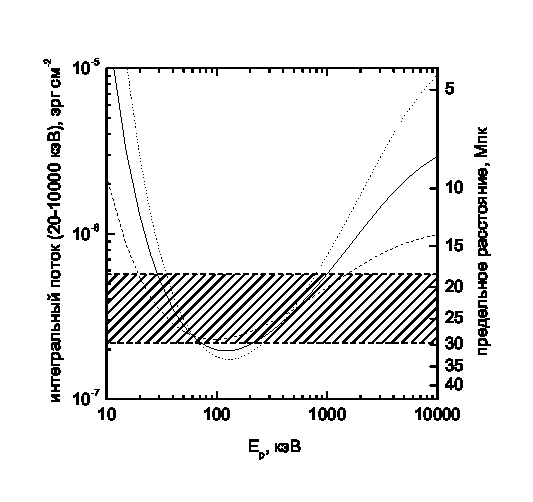
\includegraphics [width=0.8\textwidth] {gLimDist18to30RU.eps}
    \caption[Зависимость минимального интегрального потока за 140~мс 
    (20~кэВ--10~МэВ) от пиковой энергии спектра.]
    {Зависимость минимального интегрального потока за 140~мс (20~кэВ--10~МэВ) 
и предельного расстояния, в предположении энерговыделения $Q=2.3\times 10^{46}$~эрг
от параметров спектральной модели CPL $E_{\rmn{p}}$ и $\alpha$: сплошная линия~--- $\alpha=-1$, 
штриховая линия~--- $\alpha=-1.5$, пунктирная линия~--- $\alpha=-0.5$. 
Штрихованная область~--- диапазон предельных расстояний $\approx 18\textrm{--}30$~Мпк 
соответствующий диапазону $E_{\rmn{p}}\sim 250\textrm{--}1000$~кэВ.}
\end{figure}

Также была исследована зависимость площадей областей локализации IPN от потока, 
измеренного Конус-Винд в диапазоне 20~кэВ--10~МэВ на интервале 140~мс 
с наибольшей скоростью счёта, при этом не было обнаружено существенной корреляции, 
см.~рис.~\ref{img:IPN_box_area}. Таким образом, можно принять полученное 
значение $S_{\rmn{min}}$ за чувствительность IPN для коротких гамма-всплесков.

\begin{figure}[h]
    \label{img:IPN_box_area}
    \center
    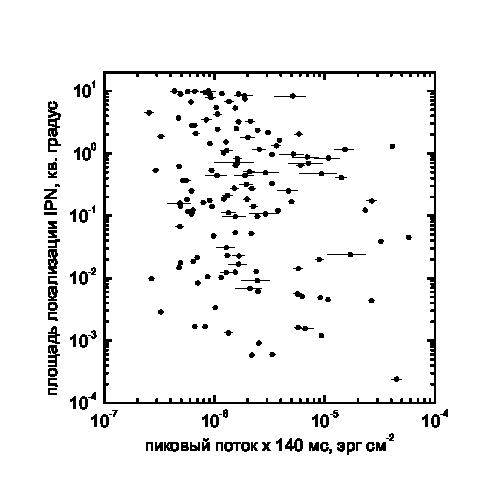
\includegraphics [width=0.8\textwidth] {gAreaVsFluenceRU.eps}
    \caption{Площадь области локализации IPN в зависимости от интегрального потока 
    (20--10000~кэВ) на интервале 140~мс с максимальной скоростью счёта.}
\end{figure}

Оценки расстояния до SGR~1806$-$20 находятся в диапазоне примерно от 6 
до~19~кпк~\citep{Tendulkar2012ApJ}, по самым последним оценкам~\citep{Svirski2011} 
диапазон расстояний составляет 9.4--18.6~кпк.

Изотропное энерговыделение начального импульса ГВ от SGR~1806$-$20 
($Q = 2.3\times 10^{46} d_{15}^2 $~эрг) предполагает предельное расстояние 
детектирования $d_{\rmn{max}} = (18\textrm{--}30)\times d_{15}$~Мпк, 
где $d_{15}=d/15$~кпк и $d$~--- расстояние до SGR~1806$-$20. 
Менее интенсивные ГВ с энерговыделением $Q \approx 10^{45}$~эрг 
(сравнимые со вспышкой 5-го марта 1979~г от SGR~0526$-$66) 
могут быть зарегистрированы до расстояний $d_{\rmn{max}} = (3.8\textrm{--}6.3) Q_{45}^{0.5}$~Мпк, 
где $Q_{45}$~--- энерговыделение вспышки в единицах $10^{45}$~эрг. 
Диапазон значений $d_{\rmn{max}}$ является трансляцией диапазона $S_{\rmn{min}}$.

\section{Набор близких галактик}\label{Gal_sample}
Наиболее полным каталогом, содержащим параметры близких галактик является 
каталог для поиска источников гравитационных волн (Gravitational Wave Galaxy Catalogue, 
GWGC~\citep{White2011CQGra}). Каталог содержит более 53000 галактик на расстояниях 
до~100~Мпк. Для поиска возможных родительских галактик гигантских вспышек SGR 
изначально был выбран набор из 8112 галактик на расстояниях до~30~Мпк. 
Неопределённость расстояний до галактик в наборе составляет 15--22\%.

Используя метод предложенный в работе~\citep{Ofek2007} была оценена полнота набора, 
связанная с затенением Галактикой. Было построено распределение галактик по Галактической 
широте с шагом $10^\circ$ разность числа галактик в интервале 
$0^\circ\textrm{--}10^\circ$ и числа галактик в незатенённом интервале 
$10^\circ\textrm{--}20^\circ$ отнесённая к общему числу галактик даёт долю 
потерянных галактик 6\% и полноту набора галактик $\epsilon_{\rmn{G}}=94$\%.

В предположении, что все SGR~--- молодые изолированные нейтронные звёзды, считалось, 
что число SGR пропорционально частоте вспышек сверхновых с коллапсом ядра 
(CCSN, типы Ib/c и~II) в галактике.

Следуя работам~\citep{Cappellaro1999, Boser2013} считалось, что частота вспышек 
сверхновых пропорциональна голубой светимости галактики ($L_{B}$) $R_{\rmn{SN}} = k L_{B}$, 
где $k$ множитель зависящий от морфологического типа галактики данный 
в единицах SNu, см.~таб.~\ref{tab:RateCCSN}. Параметры фильтра $B$: $\lambda=445$~нм 
и $\rmn{FWHM}=94$~нм~\citep{Binney1998GalAstr}.

\begin{table} [h]
  \centering
  \scriptsize
  \parbox{15cm}{\caption{Ожидаемая частота вспышек CCSN в зависимости от типа галактики}
  \label{tab:RateCCSN}}
  \begin{tabular}{ccc}
  \hline
  \hline
  Тип галактики & Числовой тип &  Частота вспышек CCSN ($k$) в SNu \\
  по Хабблу     &  по Хабблу   &           \\     
  \hline
   E-S0           &  $-6$--$-1$ &  $<0.05$ \\
   S0a-Sb         &  $0$--$3$   &  $0.89\pm0.33$ \\
   Sbc-Sd         &  $4$--$7$   &  $1.68\pm0.60$ \\
   Sm, Irr., Pec. &  $8$--$10$  &  $1.46\pm0.71$\\
  \hline
  \end{tabular}
\end{table}

Единица SNu соответствует $1\rmn{SN}(100\rmn{год})^{-1}(10^{10}L_{\odot B})^{-1}$, 
где $L_{\odot B} = 2.16\times10^{33}$~эрг~с$^{-1}$ светимость Солнца в фильтре~$B$. 
Светимость галактики $L_{B}$ вычислялась по формуле 
$L_{B}=10^{-0.4(M_B-M_{\odot B})} L_{\odot B}$, 
где $M_{\odot B}=5.48$ абсолютная звёздная величина Солнца в фильтре~$B$. 

Исходный набор 8112 галактик содержит 790 галактик, для которых не дана $L_{B}$,
таким образом полнота набора по $L_{B}$ составляет $\epsilon_{L} \approx 90$\%. 
Среди оставшихся 7322 галактик с указанным $L_{B}$, для 2405 не указан морфологический тип. 
Яркость этих галактик в среднем меньше на три звёздные величины по сравнению 
с классифицированными галактиками, при этом они содержат меньше 7\% суммарной 
частоты вспышек сверхновых, поэтому эти галактики были исключены из дальнейшего 
рассмотрения. 

В качестве итогового набора галактик был взяты 1896 галактики поздних типов 
(все кроме E и S0) с наибольшими $R_{\rmn{SN}}$, содержащие $\epsilon_{\rmn{SN}}=90$\% 
от суммарной частоты вспышек сверхновых. Плотность этих галактик на небесной сфере 
составляет 0.046~градус$^{-2}$. Суммарная частота вспышек сверхновых составляет 
$R_{\rmn{SN}}=22.8 \pm 0.4$~год$^{-1}$.

Для проверки методики определения $R_{\rmn{SN}}$, объемная плотность частоты 
вспышек сверхновых $R_{\rmn{SN}}(d)/(4/3\pi d^3)$, где $d$~--- расстояние, 
для набора 1896 галактик сравнивалась 
с нижним пределом $1.9_{-0.2}^{+0.4}\times 10^{-4}$~год$^{-1}$~Мпк$^{-3}$, 
полученным в обзоре сверхновых~\citep{Mattila2012} в галактиках ближе 15~Мпк. 
Зависимость плотности $R_{\rmn{SN}}$ от расстояния представлена на рис.~\ref{img:RateCCNvsDist}. 
Объёмная плотность, полученная на основе голубой светимости галактик согласуется в 
пределах $1 \sigma$ с наблюдаемой величиной, предполагая, что $\approx 19$\% близких CCSN 
были пропущены оптическими обзорами неба.

Объёмная плотность частоты вспышек CCSN демонстрирует значимый спад на расстояниях 
свыше $\approx 22$~Мпк, что может быть связано с падением полноты набора галактик 
на б\'{о}льших расстояниях. Для оценки объёмной частоты вспышек CCNS на расстояниях 
больших 22~Мпк было использовано среднее значение в диапазоне расстояний 
до 22~Мпк~--- $(2.74 \pm 0.18) \times 10^{-4}$~год$^{-1}$~Мпк$^{-3}$, 
ошибка дана на уровне значимости $1\sigma$.

Так же было обнаружено увеличение $R_{\rmn{SN}}/V$ внутри $\sim 10$~Мпк вплоть до 
$(9.3 \pm 0.16) \times 10^{-4}$~год$^{-1}$~Мпк$^{-3}$ внутри объёма 5~Мпк. 
При этом всего пять галактик содержат 25\% общей частоты CCSN:
GC047885 на расстоянии $d = 5$~Мпк, IC~0342 на расстоянии 3.28~Мпк, NGC~6946 на 
расстоянии 5.9~Мпк, NGC~5457~(M101) на расстоянии 6.7~Мпк и  NGC~5194~(M51) 
на расстоянии 5.9~Мпк. Эти галактики являются наиболее вероятными  источниками 
гигантских вспышек SGR в ближайшей Вселенной в дополнение к предложенным ранее 
в работе~\citep{Popov2006}: M82 на расстоянии $d = 3.4$~Мпк, NGC~253 на расстоянии 2.5~Мпк, 
NGC~4945 на расстоянии 3.7~Мпк и M83 на расстоянии 3.7~Мпк. 

\begin{figure}[h]
    \label{img:RateCCNvsDist}
    \center
    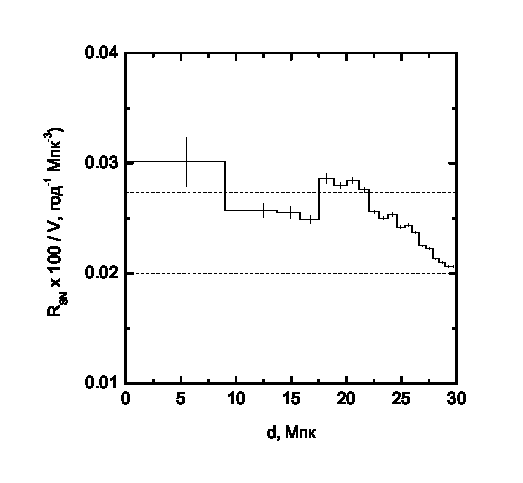
\includegraphics [width=0.8\textwidth] {gRsn2VpubRU.eps}
    \caption[Удельная частота вспышек CCSN в зависимости от расстояния]
	{Удельная частота вспышек CCSN в зависимости от расстояния $d$. 
	Сплошная линия~--- $R_{\rmn{SN}}/V(d)$ для 1896 галактик, 
	содержащих 95\% $R_{\rmn{SN}}$ внутри 30~Мпк, из каталога GWGC. 
	Горизонтальные штриховые линии обозначают $\pm 1\sigma$ интервал для 
	локальной удельной частоты вспышек сверхновых 
	$2.3_{-0.2}^{+0.5}\times 10^{-4}$~год$^{-1}$~Мпк$^{-3}$ из работы~\citep{Mattila2012}, 
    предполагая, что доля пропущенных в обзоре сверхновых составляет 0.189.}
\end{figure}

\section{Поиск гигантских вспышек среди коротких гамма-всплесков, зарегистрированных Конус-Винд}\label{GF_search}
Каталог локализаций коротких всплесков Конус-Винд, полученных при помощи 
сети IPN~\citep{Palshin2013}, содержит 271 всплеск, зарегистрированный 
по крайней мере одним КА IPN, что дало возможность локализовать их при помощи 
триангуляции (см.~Главу~\ref{chapt3}). Этот набор содержит 23 всплеска, 
классифицированные как короткие гамма-всплески с продлённым излучением.

Набор всплесков для поиска кандидатов в ГВ был ограничен 140 всплесками с 
площадями областей локализации меньше 10~кв.~градусов. После чего был произведён 
поиск галактик, накладывающихся на области локализации всплесков. При поиске наложений 
галактика моделировалась в виде круга с центром, взятым из каталога, и диаметром, 
равным большой полуоси галактики. 

Оценка ожидаемого числа галактик в этом наборе областей локализации была выполнена 
методом Монте-Карло. Было сгенерировано 1000 реализаций набора галактик, в которых 
центры галактик выбирались случайным образом. Для каждого набора вычислялось число 
наложений галактик на локализации. Полученные числа сортировались по возрастанию 
и в качестве границ 95\% доверительного интервала для числа наложений 
бралось 25-е и~975-е число.

Было обнаружено, что на 12 из 140 IPN локализаций, с общей площадью 217~кв.~градусов 
накладывается 20 галактик, при этом ни одна локализация всплеска с продлённым 
излучением не содержит галактики. Для этого набора локализаций число галактик 
ожидаемое из случайного наложения равно 22--44 на уровне значимости 95\%. 
Также было обнаружено, что локализация только одного всплеска (GRB~050312) 
накладывается на окраину скопления Девы, при этом локализация не накладывается 
ни на одну галактику из набора. Здесь скопление девы моделировалось кругом с центром в 
$\rmn{R.A.}=188^\circ$, $\rmn{Dec.}=12^\circ$ с радиусом $6^\circ$, 
параметры скопления были взяты из работы~\citep{Binggeli1987}.

Поиск наложений показал, что только два всплеска имеют малую вероятность случайного 
наложения на близкую галактику $P_{\rmn{chance}} \sim 1$\%. Эти всплески ранее были 
отнесены к внегалактическими ГВ: GRB~051103, чья локализация накладывается на группу галактик M81/M82 
(площадь бокса $4.3\times10^{-3}$~кв.~градусов) и GRB~070201, считающийся ГВ в галактике 
Андромеды (площадь бокса 0.123~кв.~градусов). Вероятность $P_{\rmn{chance}}$ 
соответствует обнаружению как минимум одной галактики в заданной локализации (боксе).

Затем процедура поиска была применена к набору 98 локализаций с площадью меньше 
1~кв.~градус, который содержит всплески, зарегистрированные по крайней мере одним 
удалённым космическим аппаратом~(см. главу~\ref{chapt3}). Было обнаружено, 
что только локализации двух упомянутых выше всплесков содержат галактики.

Общей чертой всех известных ГВ является малая длительность начального импульса 
$\lesssim 500$~мс и малое время нарастания импульса $t_{\rmn{r}} \lesssim 25$~мс. 
Среди 296 коротких всплесков 40 имеют $t_{\rmn{r}}<25$~мс и длительность $<500$~мс. 
Ранее обнаруженные кандидаты GRB~051103 и GRB~070201 имеют $t_{\rmn{r}}=2$~мс 
и~$t_{\rmn{r}}=24$~мс соответственно. Ограничив набор всплесков 17-ю с площадями 
областей локализации менее 10~кв.~градусов, было обнаружено, что четыре области 
локализации с общей площадью 47~кв.~градусов накладываются на пять галактик. 
Это число согласуется с ожидаемым из случайного наложения 5--16 галактик. Из этих 
четырёх всплесков только GRB~051103 и GRB~070201 имеют малые вероятности случайного наложения.
Результаты поиска наложений для всех перечисленных наборов всплесков приведены 
в Таблице~\ref{tab:SearchResults}.

\begin{table}[h]
  \centering
  \scriptsize
  \caption{Результаты поиска кандидатов в гигантские вспышки SGR в 
  наборе коротких всплесков Конус-Винд}
  \label{tab:SearchResults}
  \begin{tabular}{cccc}
  \hline
  \hline
Описание & Число локализаций  & Число галактик & Ожидаемое число  \\
набора   &                    & в локализациях & наложений на уровне 95\% \\
\hline
Площадь локализации $<10$~кв.~градусов  & 140 & 20 & 22--44 \\
Площадь локализации $<1$~кв.~градусов   & 98 & 2 & 0--7\\
$t_{\rmn{r}} \leq 25$~мс, $T_{100}<500$~мс, & 17 & 5 & 5--16\\
и площадь локализации $<10$~кв.~градусов & & & \\
\hline
\end{tabular}
\end{table}

С учетом произведения факторов полноты набора галактик $\epsilon_{\rmn{G}} \epsilon_{\rmn{L}} \epsilon_{\rmn{SN}} \approx 76$\%, 
и предполагая, что было найдено два кандидата в ГВ среди 98 хорошо локализованных коротких всплесков, 
можно поставить верхний предел на долю ГВ среди коротких всплесков Конус-Винд 
$<8$\% (=6.296/98/0.76), где 6.296~--- 95\% односторонний верхний предел на 
число вспышек~\citep{Gehrels1986}. Благодаря непрерывному наблюдению всего неба IPN 
этот предел может быть распространён на всю популяцию коротких гамма-всплесков с 
интегральными потоками выше $\sim 5\times 10^{-7}$~эрг~см$^{-2}$. Полученный верхний 
предел жестче чем полученный в работе~\citep{Ofek2007}.

\section{Верхний предел на частоту гигантских вспышек}\label{GF_rate}
Предполагая, что только одна ГВ с энерговыделением $Q \gtrsim 10^{46}$~эрг наблюдалась 
в группе галактик M81/M82 внутри объёма $d \le 30$~Мпк, можно получить верхний предел 
на частоту подобных ГВ. Предполагая, что число активных SGR ($N_{\rmn{SGR}}(d)$) 
внутри сферы радиуса $d$ пропорционально частоте вспышек CCSN 
$R_{\rmn{SN}}(d)=4/3 \pi d^3 r_{\rmn{SN}}$, где $r_{\rmn{SN}}$~--- объёмная частота вспышек CCSN.
\begin{equation}\label{eq:NumSGR}
N_{\rmn{SGR}} (d) = \frac{N_{\rmn{SGR}, \rmn{MW+LMC}}}{ R_{\rmn{SN}, \rmn{MW+LMC}}} R_{\rmn{SN}}(d).
\end{equation}
Галактическая частота CCSN равна $R_{\rmn{SN}, \rmn{MW}} = 0.028\pm0.006$~в~год 
с систематической ошибкой $\sim 2$~раза~\citep{Li2011part3}, и частотой в Большом 
Магеллановом облаке (LMC)~$R_{\rmn{SN}, \rmn{LMC}} = 0.013\pm0.009$~в~год~\citep{Bergh1991}. 
Таким образом, суммарная частота равна $R_{\rmn{SGR}, \rmn{MW+LMC}} = 0.041\pm0.011$~в~год. 

Наблюдаемая частота гигантских вспышек на SGR задаётся выражением
\begin{equation}\label{eq:RateGF}
R_{\rmn{GF}} = \frac{N_{\rmn{GF},\rmn{obs}}}{\Delta T N_{\rmn{SGR}}(d_{\rmn{max}})} ,
\end{equation}
где $N_{\rmn{GF},\rmn{obs}}$~--- число зарегистрированных ГВ, 
$\Delta T=16$~лет~--- время наблюдения Конус-Винд и $N_{\rmn{SGR}}(d_{\rmn{max}})$ 
задано уравнением~\ref{eq:NumSGR}. Для оценки верхнего предела на $R_{\rmn{GF}}$ 
в случае одной зарегистрированной ГВ использовался 95\% односторонний верхний предел
на $N_{\rmn{GF}, \rmn{obs}}=4.744$~\citep{Gehrels1986}.

Для частоты ГВ с энерговыделением $Q \gtrsim 10^{46}$~эрг в объеме $d\le30$~Мпк уравнение~\ref{eq:RateGF} 
даёт верхний предел ${(0.6\textrm{--}1.2)\times 10^{-4} Q_{46}^{-1.5}}$~год$^{-1}$~SGR$^{-1}$, 
где $Q_{46}$ энерговыделение ГВ в единицах $10^{46}$~эрг. Диапазон верхнего предела 
является трансляцией ошибок частоты вспышек CCSN. Регистрация только 
одной ГВ с энерговыделением $Q \gtrsim 10^{46}$~эрг за последние 35~лет 
с 1979~г от SGR~1806$-$20 предполагает частоту таких вспышек в галактике 
${(0.005\textrm{--}1)\times 10^{-2}}$~год$^{-1}$~SGR$^{-1}$ ($=1_{-0.98}^{+4.6} / 35 / 15 $) 
для одностороннего 95\% уровня значимости. Это величина согласуется с верхним пределом, 
вычисленным выше с учётом диапазона расстояний до SGR~1806$-$20 9.4--18.6~кпк, 
в основном из за больших неопределённостей в галактической частоте ГВ. 

Для менее интенсивных ГВ с энерговыделением $Q \lesssim 10^{45}$~эрг, которые 
могут регистрироватся Koнуc-Винд и IPN на расстояниях до 6.3~Мпк, считая что 
одна такая вспышка была зарегистрирована из галактики Андромеды, верхний предел 
на частоту вспышек составляет
${(0.9\textrm{--}1.7)\times 10^{-3}}$~год$^{-1}$~SGR$^{-1}$. Этот предел согласуется
с наблюдаемой галактической частотой таких вспышек 
${(0.5\textrm{--}1.4)\times 10^{-2}}$~год$^{-1}$~SGR$^{-1}$. Верхний предел и 
интервал галактической частоты ГВ дан на уровне значимости 95\%.

\section{Заключение}\label{Summary}
В этой главе была оценена чувствительность Конус-Винд и IPN, и было получено 
предельное расстояние регистрации гигантских вспышек SGR схожих с ГВ от SGR~1806$-$20 
равное $(18\textrm{--}30) d_{15}$~Мпк. Показано, что менее интенсивные ГВ, сравнимые 
с ГВ от SGR~1900+14 и SGR~0526$-$66 могут быть зарегистрированы в галактиках 
не далее $\approx 6$~Мпк.

Был произведён поиск близких галактик, находящихся ближе 30~Мпк, в локализациях 
коротких гамма-всплесков Конус-Винд. Были обнаружены только два всплеска, ранее 
ассоциированые с группой галактик M81/M82 (GRB~051103) и галактикой Андромеды (GRB~070201),
локализации которых имеют малую вероятность случайного наложения на эти галактики.
Дополнительный поиск всплесков из скопления Девы не выявил возможных кандидатов в ГВ.

Полученный верхний предел на частоту ГВ с энегрговыделением $Q \gtrsim 10^{46}$~эрг равный
${(0.6\textrm{--}1.2)\times 10^{-4} Q_{46}^{-1.5}}$~год$^{-1}$~на~SGR, предполагает 
около одной ГВ с таким энерговыделением за время активности SGR, $10^3\textrm{--}10^5$~лет. 
Этот предел был вычислен на основе наибольшего на сегодняшний момент (2014~г) 
набора коротких всплесков и согласуется с ранее полученной в работе~\citep{Ofek2007} оценкой.
 
Для ГВ, сопоставимых по энерговыделению со вспышкой 5-го марта~1979~г ($Q \lesssim 10^{45}$~эрг), 
полученный верхний предел на порядок выше $(0.9\textrm{--}1.7)\times 10^{-3}$~yr$^{-1}$~SGR$^{-1}$. 
Что может быть интерпретировано, как возможность наблюдать более одной подобной ГВ за время жизни SGR.
Измеренное дипольное магнитное поле SGR~1900+14 и SGR~0526$-$66, 
$5.6\times10^{14}$~Гс и $7\times10^{14}$~Гс, соответственно~\citep{Olausen_Kaspi2014}, 
по-видимому, является достаточным для генерации десятка ГВ с энерговыделением $Q \sim 10^{45}$~erg.

Полученные верхние пределы содержат неопределённость в порядок величины, связанную с
неопределённостью галактической частоты вспышек CCSN, расстояния до SGR~1806$-$20 и
предельного расстояния детектирования IPN.

Определены галактики, которые являются наиболее вероятными источниками ГВ 
из-за наибольшего оцененного количества SGR в этих галактиках. Это галактики
PGC047885, IC~0342, NGC~6946, NGC~5457 и NGC~5194, в дополнении к предложенным 
в работе~\citet{Popov2006}.

Дополнительно был вычислен верхний предел на частоту ярких ГВ с использованием 
данных \textit{Swift}-BAT. С момента запуска в ноябре 2004~г \textit{Swift} наблюдал 
только один кандидат в ГВ, GRB~050906~\citep{Levan2008}, предположительно из 
галактики IC~328 на расстоянии $\approx 130$~Мпк. Этот всплеск имел наименьший 
интегральный поток в диапазоне 15--150~кэВ из всех зарегистрированных на 2011~г всплесков, 
$S_{\rmn{min}} = 6.1\times10^{-9}$~эрг~см$^{-2}$~\citep{Sakamoto2011ApJS} и 
мягкий спектр, описывающийся степенным законом с показателем~$-1.7$. Экстраполяция 
энерговыделения ГВ от SGR~1806$-$20 из диапазона 10~кэВ--10~МэВ в 15--150~кэВ, 
используя степенной закон с экспоненциальным завалом с параметрами $\alpha=-0.73$ 
и $E_{\rmn{p}}=850$~keV даёт $2.5\times10^{45}$~эрг, что соответствует предельному 
расстоянию детектирования 60~Мпк. Полученное предельное расстояние детектирования 
в совокупности с мягким спектром всплеска делает ассоциацию с SGR в IC~328 маловероятной.

Время наблюдения 90\% неба BAT в 2004--2010~гг 
составило $7.25\times10^{6}$~с (0.23~года)~\citep{Baumgartner2013ApJS}, и экстраполяция 
этой величины на 2004--2013~гг даёт 0.35~лет. Отсутствие зарегистрированных ГВ в 
объеме $d \lesssim 60$~Мпк в течении наблюдений \textit{Swift}-BAT даёт верхний предел 
на частоту ГВ на уровне 95\% $\sim 6 \times 10^{-4} Q_{45}^{-1.5} $~год$^{-1}$~на~SGR, 
где $Q_{45}$~--- энерговыделение ГВ в единицах $10^{45}$~эрг в диапазоне 15--150~кэВ. 
Таким образом не смотря на высокую чувствительность BAT, полученный предел 
менее жесткий чем полученный по данным Конус-Винд и IPN из-за меньшего экспозиции всего неба.

\clearpage